\documentclass[12pt]{article}
\usepackage[utf8]{inputenc}
\usepackage[spanish]{babel}
\usepackage{geometry}
\usepackage{hyperref}
\usepackage{graphicx}
\usepackage{xcolor}
\usepackage{listings}
\usepackage{booktabs}
\geometry{letterpaper, margin=2.5cm}

% Estilo para el código Python
\lstdefinestyle{mypython}{
    language=Python,
    basicstyle=\ttfamily\small,
    keywordstyle=\color{blue}\bfseries,
    stringstyle=\color{red},
    commentstyle=\color{green!50!black},
    breaklines=true,
    showstringspaces=false,
    numbers=left,
    numberstyle=\tiny\color{gray},
    frame=single,
    backgroundcolor=\color{gray!10}
}

\begin{document}

% Portada con logos
\begin{minipage}{0.25\textwidth}
    
\includegraphics[width=3cm]{unam.png}
\end{minipage}
\begin{minipage}{0.5\textwidth}
    \begin{center}
        \Large \textbf{Universidad Nacional Autónoma de México} \\[0.3cm]
        \normalsize Facultad de Ingeniería \\
        Sistemas Operativos
    \end{center}
\end{minipage}
\begin{minipage}{0.25\textwidth}
    \raggedleft
    
\includegraphics[width=3cm]{fi.png}
\end{minipage}

\vspace{1.5cm}

\begin{center}
    \textbf{Grupo: 8} \\[0.3cm]
    \textbf{Tarea: 2 Comparación de Planificadores} \\[1cm]
    \textbf{Integrante:} \\[0.3cm]
    321101464 Michelle Ariana Castañeda González
\end{center}

\vspace{1.5cm}

\section*{Comparación de planificadores}

En la tarea se compararon distintos mecanismos de planificación de procesos del sistema operativo, bajo diferentes cargas aleatorias de trabajo, para analizar su comportamiento y rendimiento. 

Se desarrolló un programa en Python denominado \texttt{tarea\_planificadores.py}, que implementa los siguientes algoritmos:

\begin{itemize}
    \item FCFS (First Come First Served / FIFO)
    \item RR (Round Robin) con quantum variable (\(q=1\) y \(q=4\))
    \item SPN (Shortest Process Next), versión no expropiativa de SJF
    \item FB (Feedback multinivel) con tres colas de prioridad
    \item SRR (Selfish Round Robin) o ronda egoísta, que prioriza procesos nuevos
\end{itemize}

El programa genera aleatoriamente varias rondas para después calcular las métricas promedio de cada algoritmo y muestra la ejecución mediante un diagrama de Gantt textual. Además, se comprobó manualmente la coherencia de los resultados obtenidos. 

\section*{Descripción del programa}

El simulador fue desarrollado en Python 3.11. El código es completamente portable y se ha probado en macOS. No requiere instalación de paquetes adicionales ni configuraciones externas.  

Para ejecutar el programa desde terminal:

\begin{verbatim}
python3 tarea_planificadores.py
\end{verbatim}

El programa utiliza estructuras básicas como colas (\texttt{deque}), tuplas (\texttt{namedtuple}) y diccionarios para controlar tiempos de llegada, ráfagas y estados de ejecución.

\section*{Estructura del código}

\subsection*{1. Generación de procesos}

La función \texttt{generar\_ronda()} crea listas de procesos con:

\begin{itemize}
    \item Nombre (A, B, C…)
    \item Tiempo de llegada aleatorio
    \item Ráfaga de CPU aleatoria
\end{itemize}

Cada ronda simula una carga de trabajo diferente, incluyendo posibles huecos de CPU.

\subsection*{2. Cálculo de métricas}

La función \texttt{calcular\_metricas()} obtiene para cada proceso:

\begin{itemize}
    \item T (Turnaround): tiempo desde la llegada hasta finalizar
    \item E (Espera): tiempo en cola antes de ejecutarse
    \item P (Penalización): relación entre T y ráfaga
\end{itemize}

También calcula el promedio de cada métrica para comparar algoritmos.

\subsection*{3. Planificadores}

\begin{itemize}
    \item \textbf{FCFS (First Come First Served):} ejecuta procesos en orden de llegada, sin interrupciones.
    \item \textbf{RR (Round Robin):} ejecuta procesos en cola circular por un quantum fijo; si no terminan, regresan al final. Quantum configurable (\(q=1\) o \(q=4\)).
    \item \textbf{SPN (Shortest Process Next):} selecciona el proceso con menor ráfaga entre los listos, no expropiativo.
    \item \textbf{FB (Feedback multinivel):} tres colas de prioridad (RR1, RR2, FCFS). Los procesos nuevos empiezan en la más alta; si no terminan, se degradan.
    \item \textbf{SRR (Selfish Round Robin):} procesos recién llegados se insertan al frente de la cola, obteniendo preferencia; quantum base = 2.
\end{itemize}

\section*{Ejecución}

Cada algoritmo genera un diagrama de Gantt y calcula las métricas de los procesos. Se pueden ejecutar múltiples rondas para comparar resultados.  

El programa ejecutó cinco rondas aleatorias con distintas cargas de trabajo. En cada una se muestran las métricas promedio (T, E, P) y el diagrama de Gantt.  
\begin{center}
    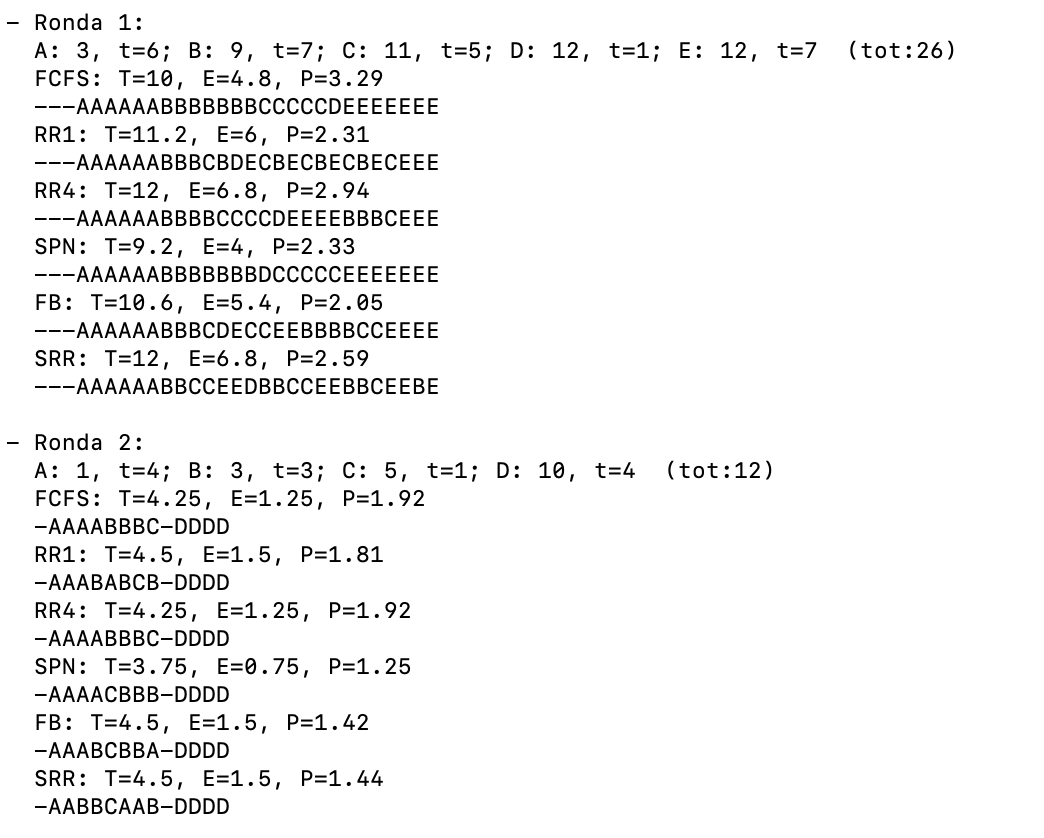
\includegraphics[width=0.9\textwidth]{ronda1.png}
\end{center}

\begin{center}
    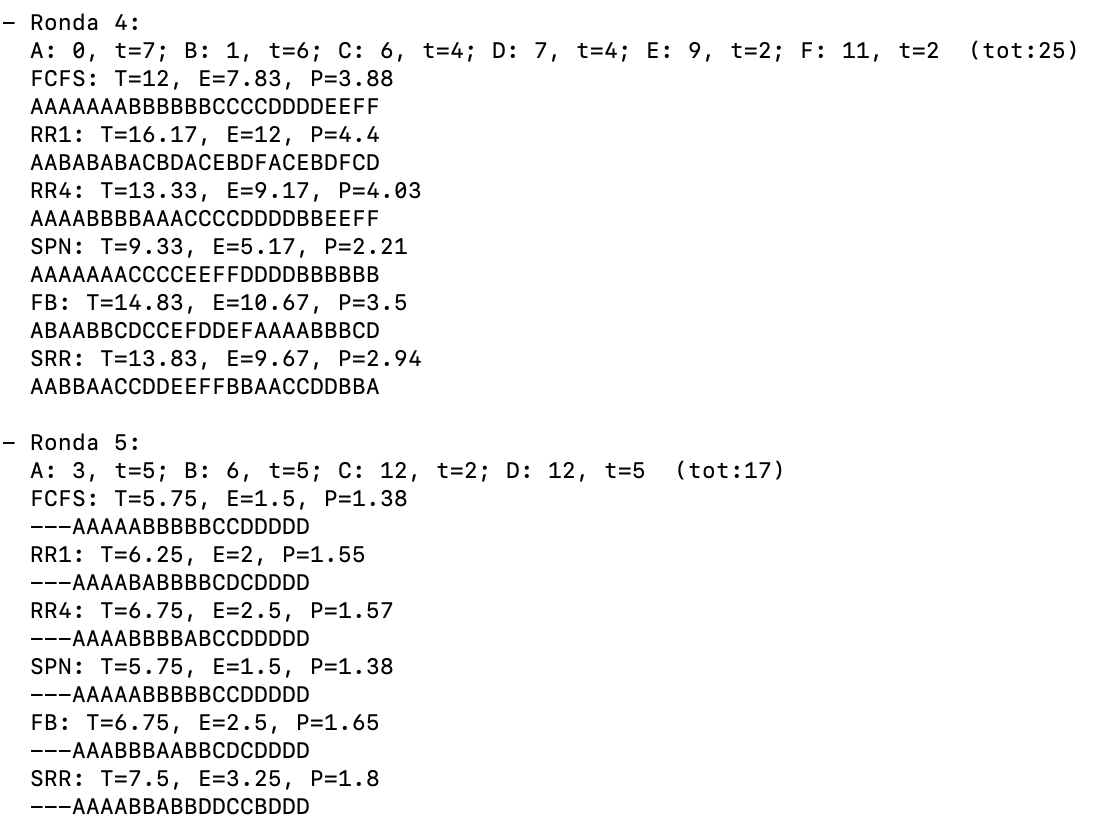
\includegraphics[width=0.9\textwidth]{ronda4.png}
\end{center}


\section*{Verificación manual}

Se revisaron manualmente las rondas 1 y 5, y los cálculos de T, E y P coincidieron con los promedios del programa.  

Los periodos de inactividad (–) y los diagramas de Gantt son correctos según cada planificador.

Procesos: A: 3, t=6; B: 9, t=7; C: 11, t=5; D: 12, t=1; E: 12, t=7.  
Carga total: 26 unidades de tiempo.  

\subsection*{FCFS (First Come First Served)}

Gantt: \texttt{---AAAAAABBBBBBBCCCCCDEEEEEEE}

\begin{center}
\begin{tabular}{lcccccc}
\toprule
\textbf{Proceso} & \textbf{Llegada} & \textbf{Ráfaga} & \textbf{Finalización} & \textbf{T} & \textbf{E} & \textbf{P} \\
\midrule
A & 3 & 6 & 9 & 6 & 0 & 1.00 \\
B & 9 & 7 & 16 & 7 & 0 & 1.00 \\
C & 11 & 5 & 21 & 10 & 5 & 2.00 \\
D & 12 & 1 & 22 & 10 & 9 & 10.00 \\
E & 12 & 7 & 29 & 17 & 10 & 2.43 \\
\midrule
\textbf{Promedio} & & & & 10.00 & 4.80 & 3.29 \\
\bottomrule
\end{tabular}
\end{center}

Coincide también con la salida del programa: FCFS: T=10, E=4.8, P=3.29

\subsection*{RR(q=1)}

Gantt: \texttt{---AAAAAABBBCBDECBECBECBECEEE}

\begin{center}
\begin{tabular}{lcccccc}
\toprule
\textbf{Proceso} & \textbf{Llegada} & \textbf{Ráfaga} & \textbf{Finalización} & \textbf{T} & \textbf{E} & \textbf{P} \\
\midrule
A & 3 & 6 & 9 & 6 & 0 & 1.00 \\
B & 9 & 7 & 24 & 15 & 8 & 2.14 \\
C & 11 & 5 & 26 & 15 & 10 & 3.00 \\
D & 12 & 1 & 15 & 3 & 2 & 3.00 \\
E & 12 & 7 & 29 & 17 & 10 & 2.43 \\
\midrule
\textbf{Promedio} & & & & 11.20 & 6.00 & 2.31 \\
\bottomrule
\end{tabular}
\end{center}

Coincide también con la salida del programa: RR1: T=11.2, E=6, P=2.31

\section*{Ronda 5}

Procesos: A: 1, t=4; B: 3, t=3; C: 5, t=1; D: 10, t=4.  
Carga total: 12 unidades de tiempo.  

\subsection*{SPN (Shortest Process Next)}

Gantt: \texttt{-AAAACBBB-DDDD}

\begin{center}
\begin{tabular}{lcccccc}
\toprule
\textbf{Proceso} & \textbf{Llegada} & \textbf{Ráfaga} & \textbf{Finalización} & \textbf{T} & \textbf{E} & \textbf{P} \\
\midrule
A & 1 & 4 & 5 & 4 & 0 & 1.00 \\
B & 3 & 3 & 9 & 6 & 3 & 2.00 \\
C & 5 & 1 & 6 & 1 & 0 & 1.00 \\
D & 10 & 4 & 14 & 4 & 0 & 1.00 \\
\midrule
\textbf{Promedio} & & & & 3.75 & 0.75 & 1.25 \\
\bottomrule
\end{tabular}
\end{center}

Coincide también con la salida del programa: SPN: T=3.75, E=0.75, P=1.25

\section*{Conclusión}

Los algoritmos no expropiativos (FCFS, SPN) generan menos cambios de contexto, mientras que RR, FB y SRR ofrecen más equidad y mejor respuesta.  

SPN logra los mejores tiempos promedio con cargas ligeras, y RR y FB equilibran bien el rendimiento en cargas mixtas.  

Tras comparar las métricas promedio con las salidas del simulador, se confirma que los resultados obtenidos por el programa son consistentes, reproducibles y lógicos según la teoría.

\end{document}
